\chapter{\appendixname}

\section*{\BdKstee \textit{Stripping17b}}
\label{ap:strip17}
\begin{figure}[!h]
\begin{center}
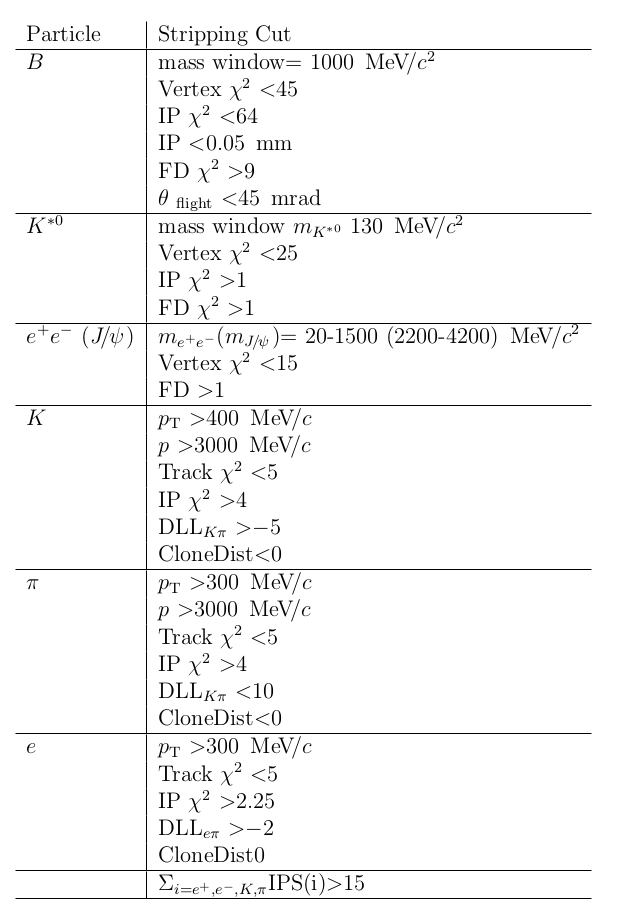
\includegraphics[width = 0.7\textwidth]{stripping17.jpg}
\end{center}
\label{stripping17}
\caption{The cuts of the 2011 \BdKstee stripping-line.}
\end{figure}
\newpage

\section*{All BDT Input Variables}
\label{ap:allvars}
\begin{figure}[!h]
\begin{center}
\subfigure{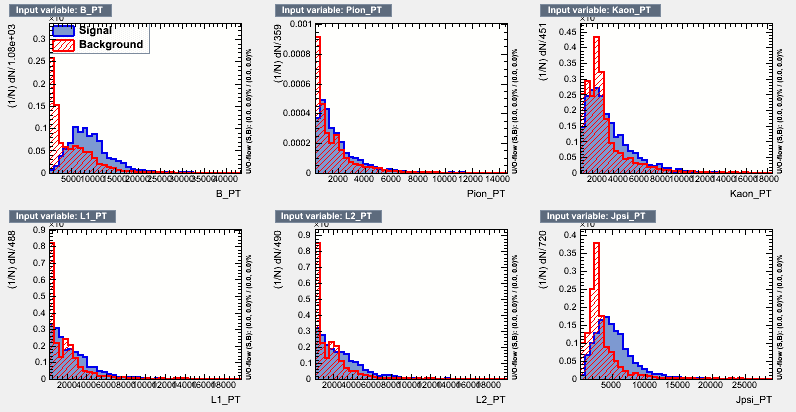
\includegraphics[width = \textwidth]{varb1.png}}
\subfigure{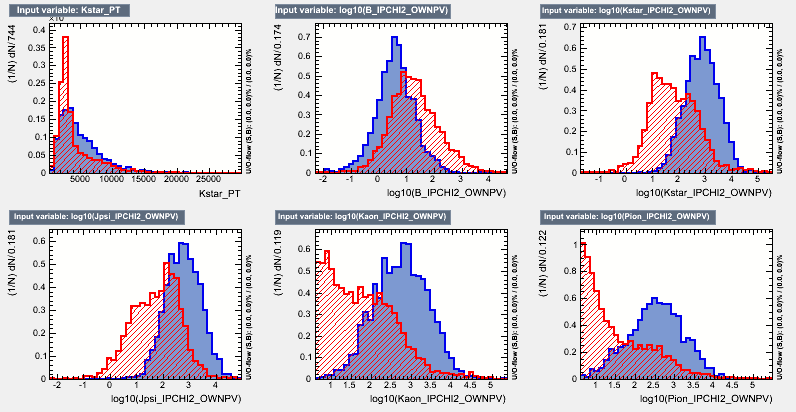
\includegraphics[width = \textwidth]{varb2.png}}
\end{center}
\label{fig:varBDTa}
\caption{\textit{Distributions for the different input variables for the \bdta training. Red distribution: background sample, blue distribution: signal sample.}}
\end{figure}
\newpage
\begin{figure}[!h]
\begin{center}
\subfigure{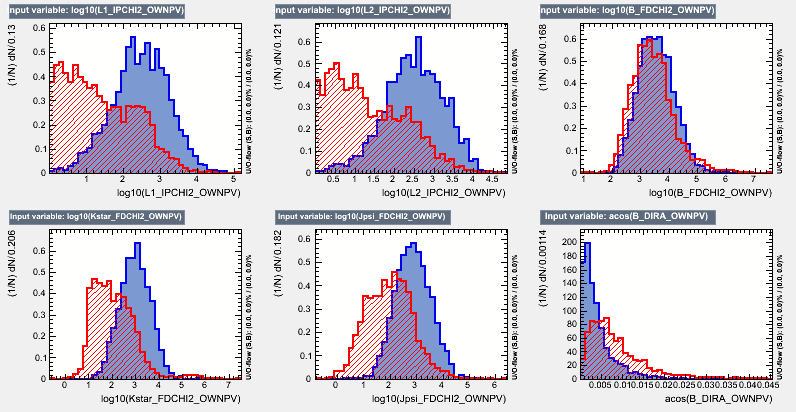
\includegraphics[width = \textwidth]{varb3.png}}
\subfigure{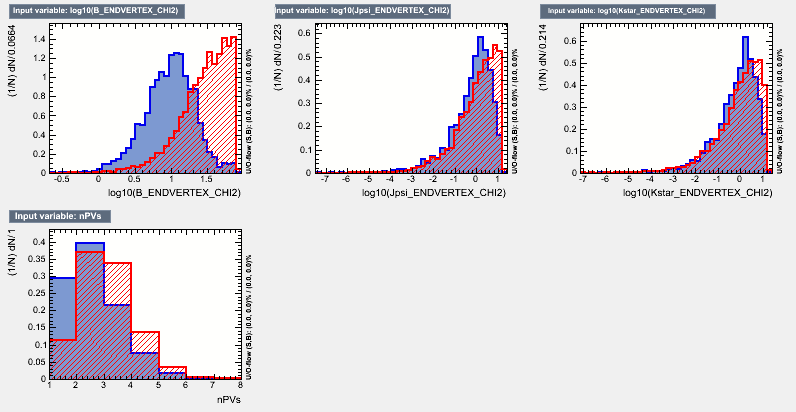
\includegraphics[width = \textwidth]{varb4.png}}
\end{center}
\label{fig:varBDTa2}
\caption{\textit{Distributions for the different input variables for the \bdta training. Red distribution: background sample, blue distribution: signal sample.}}
\end{figure}

\newpage

\begin{figure}[!h]
\begin{center}
\subfigure{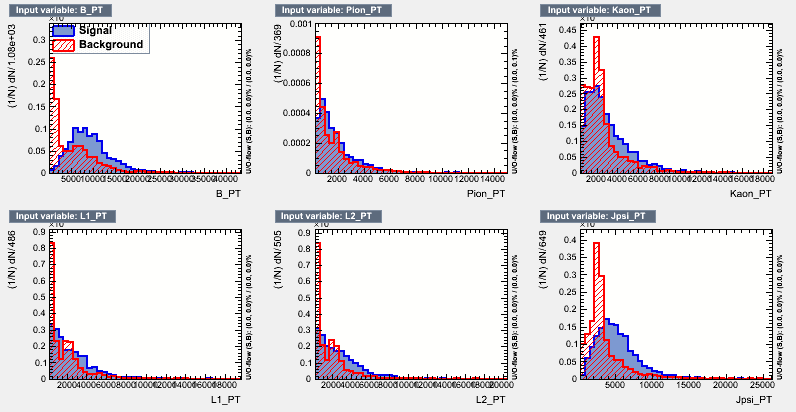
\includegraphics[width = \textwidth]{vara1.png}}
\subfigure{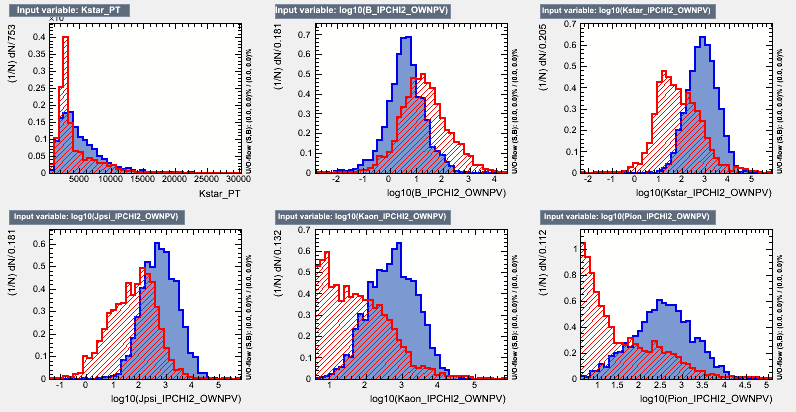
\includegraphics[width = \textwidth]{vara2.png}}
\end{center}
\label{fig:varBDTa}
\caption{\textit{Distributions for the different input variables for the \bdtb training. Red distribution: background sample, blue distribution: signal sample.}}
\end{figure}
\vspace*{5cm}
\begin{figure}[!h]
\begin{center}
\subfigure{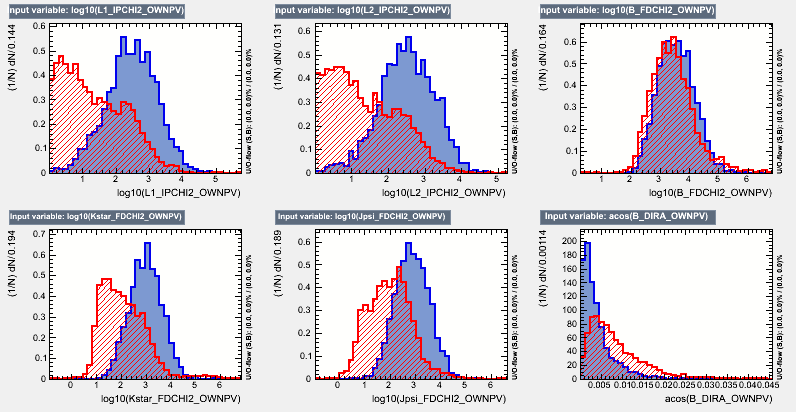
\includegraphics[width = \textwidth]{vara3.png}}
\subfigure{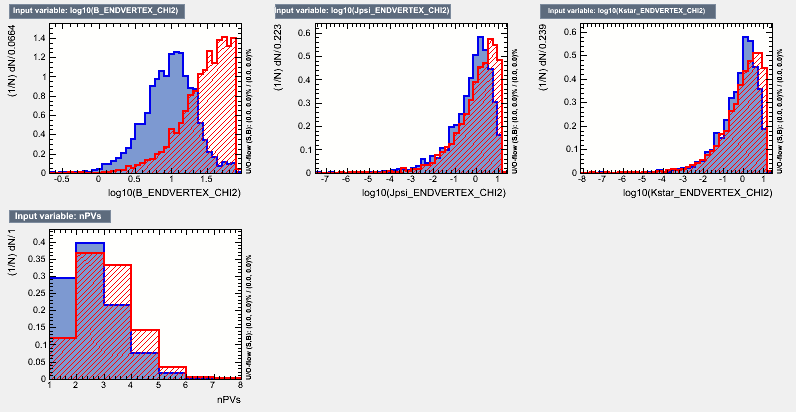
\includegraphics[width = \textwidth]{vara4.png}}
\end{center}
\label{fig:varBDTa2}
\caption{\textit{Distributions for the different input variables for the \bdtb training. Red distribution: background sample, blue distribution: signal sample.}}
\end{figure}

\vspace*{5cm}

\section*{Distribution of S and B in the optimisation process}
\label{ap:SandB}

\begin{figure}[!h]
\begin{center}
\subfigure{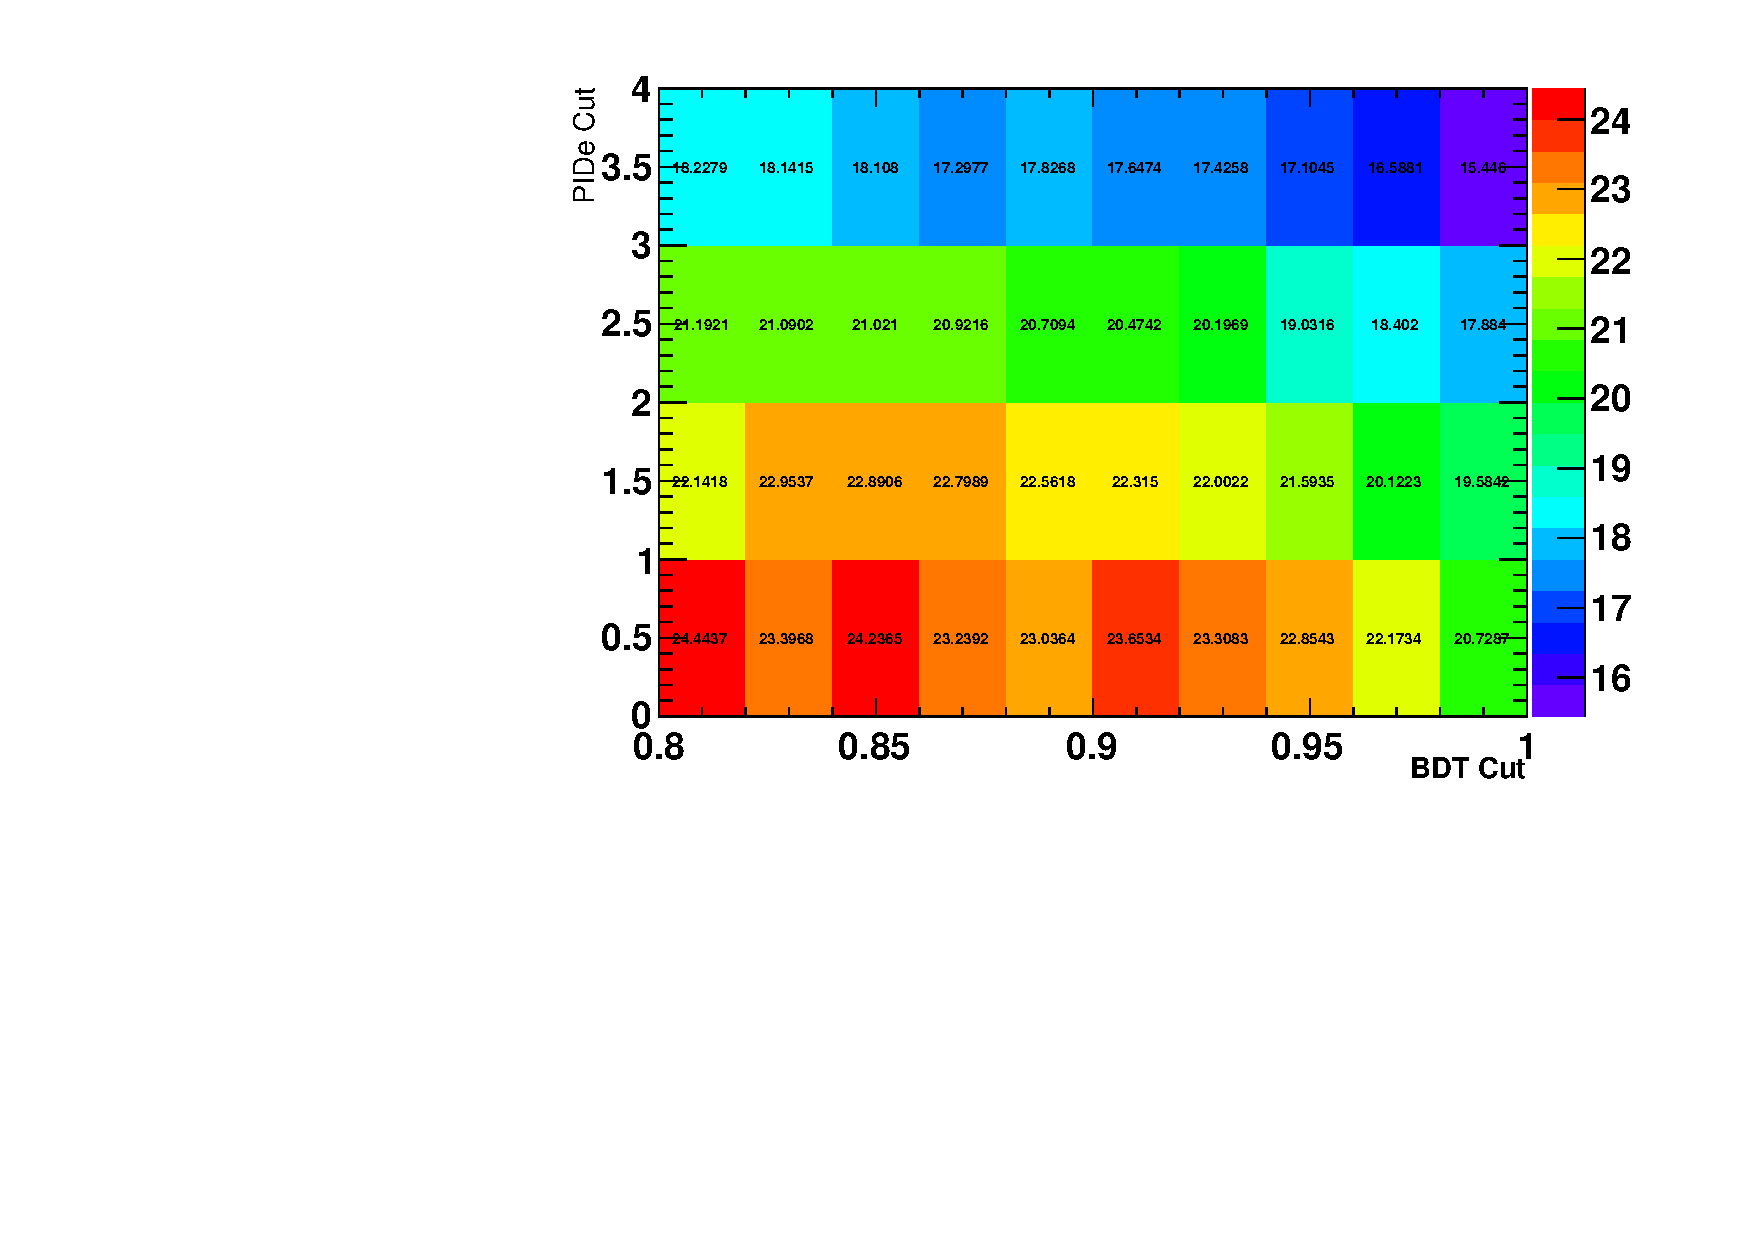
\includegraphics[width = 0.7\textwidth]{BDT_L0Ele_S.pdf}}
\subfigure{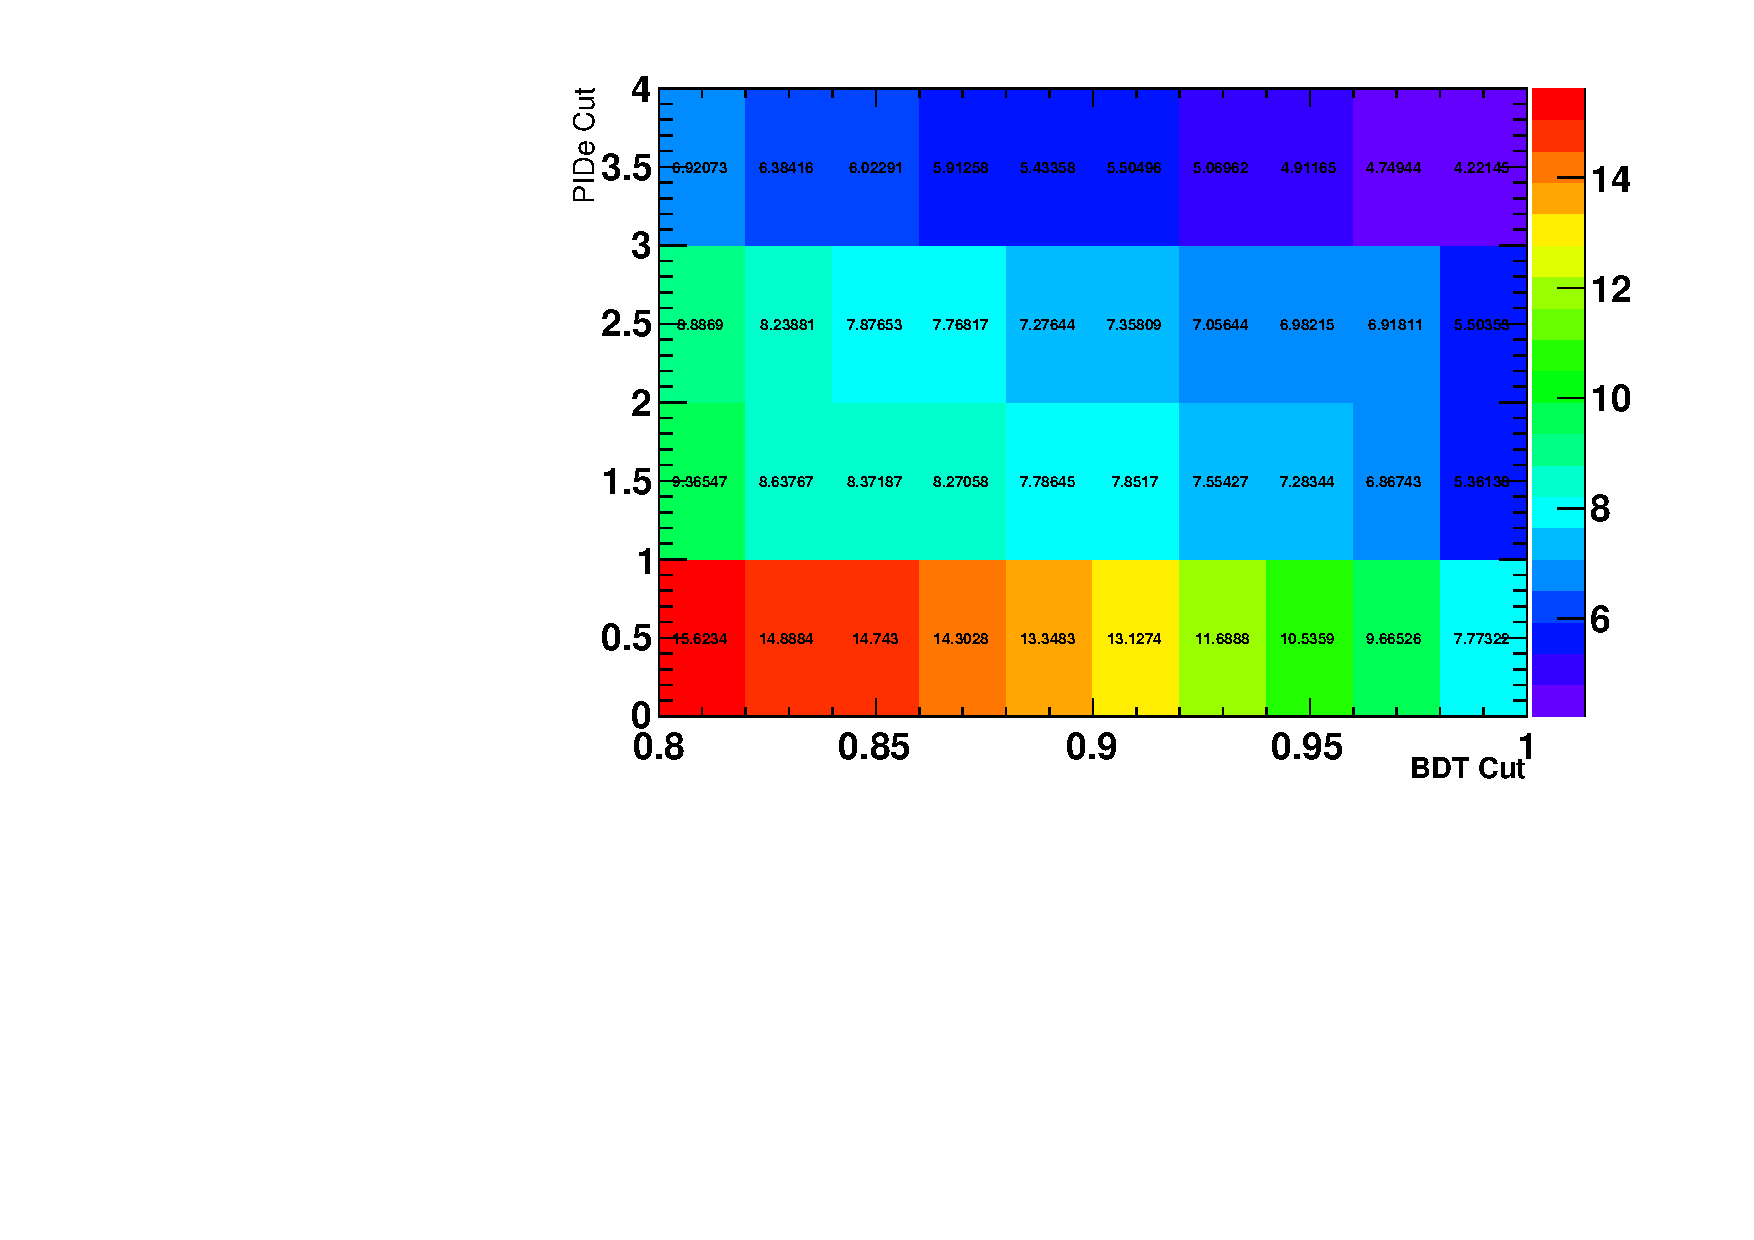
\includegraphics[width = 0.7\textwidth]{BDT_L0Ele_B.pdf}}
\end{center}
\label{fig:SBEle}
\caption{\textit{Values for the expected signal yield (top) and number of background events in the signal window (bottom) for the L0Electron trigger categories for a fourth of the 2011 and 2012 \lhcb data.}}
\end{figure}

\begin{figure}[!h]
\begin{center}
\subfigure{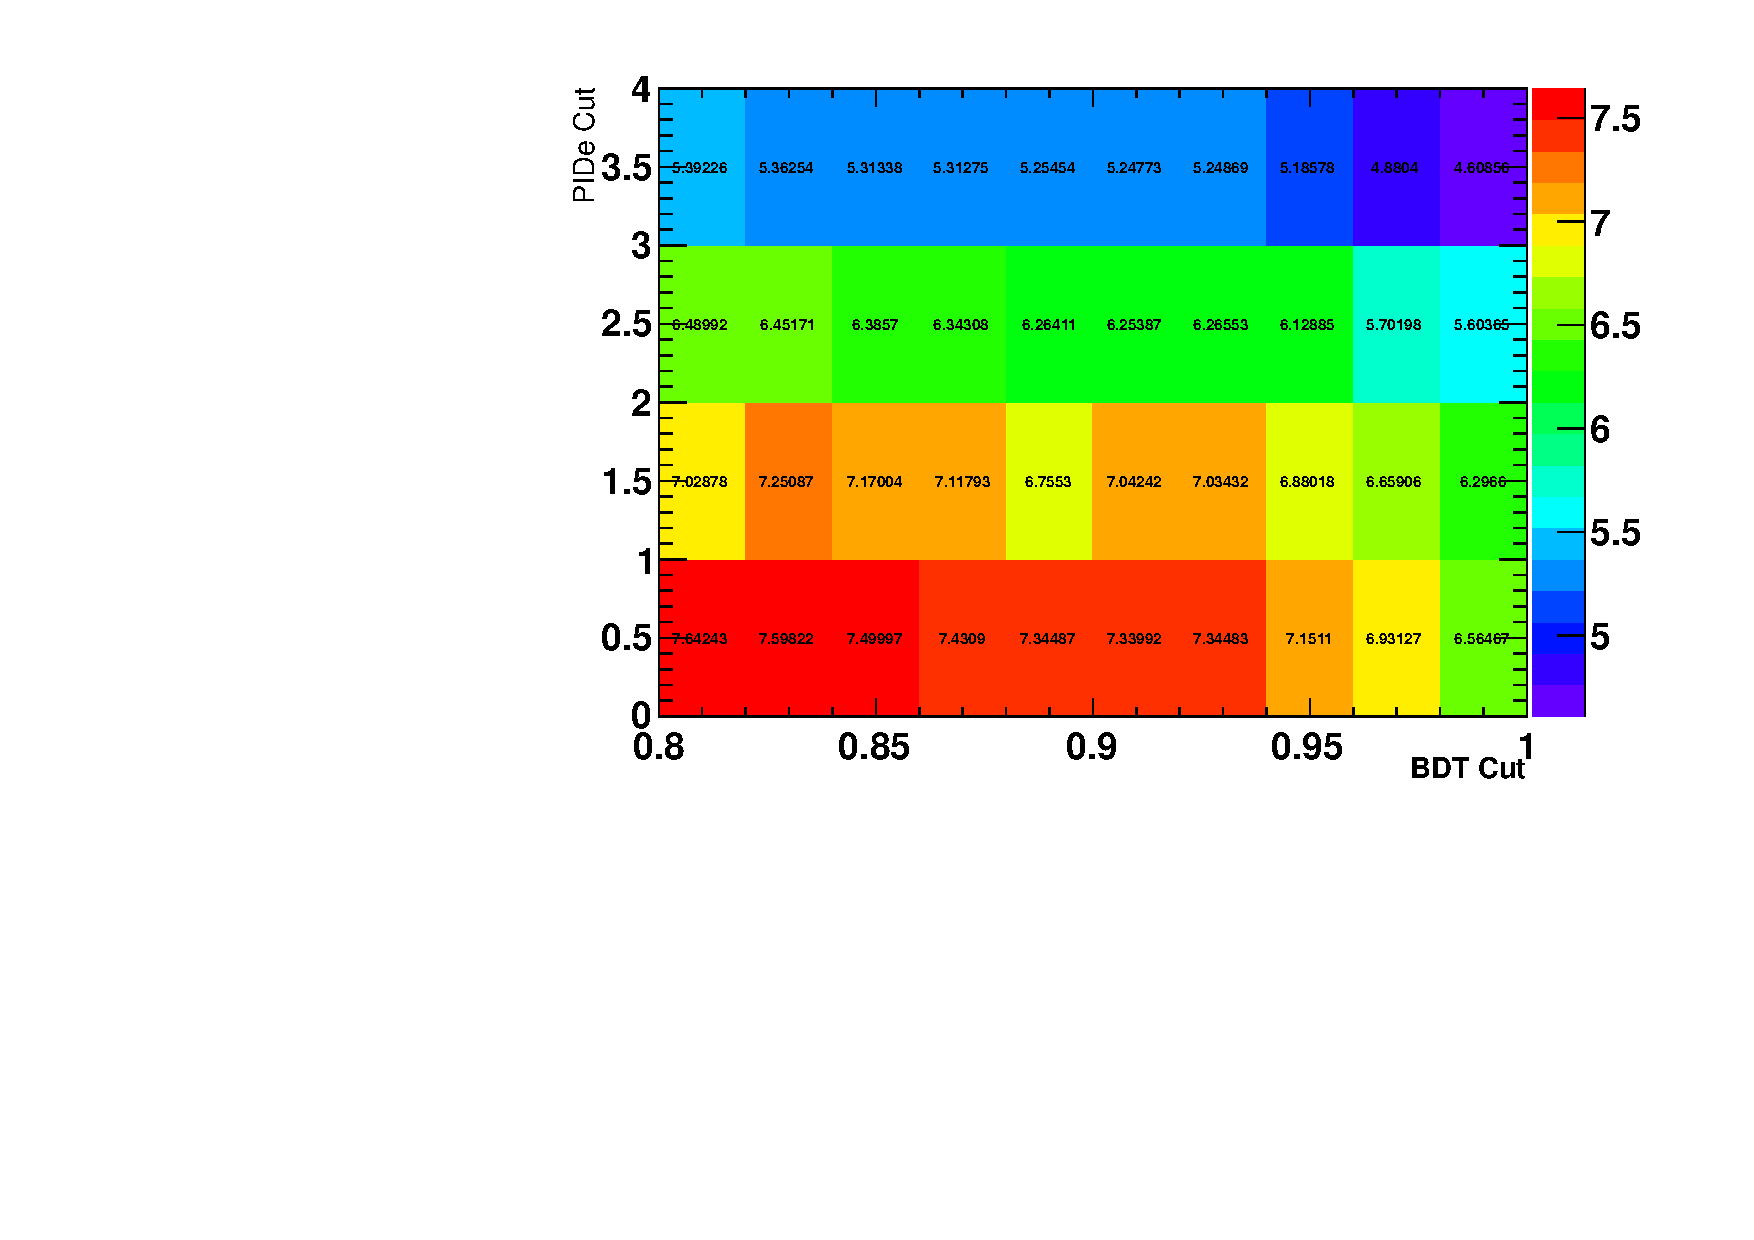
\includegraphics[width = 0.7\textwidth]{BDT_L0Had_S.pdf}}
\subfigure{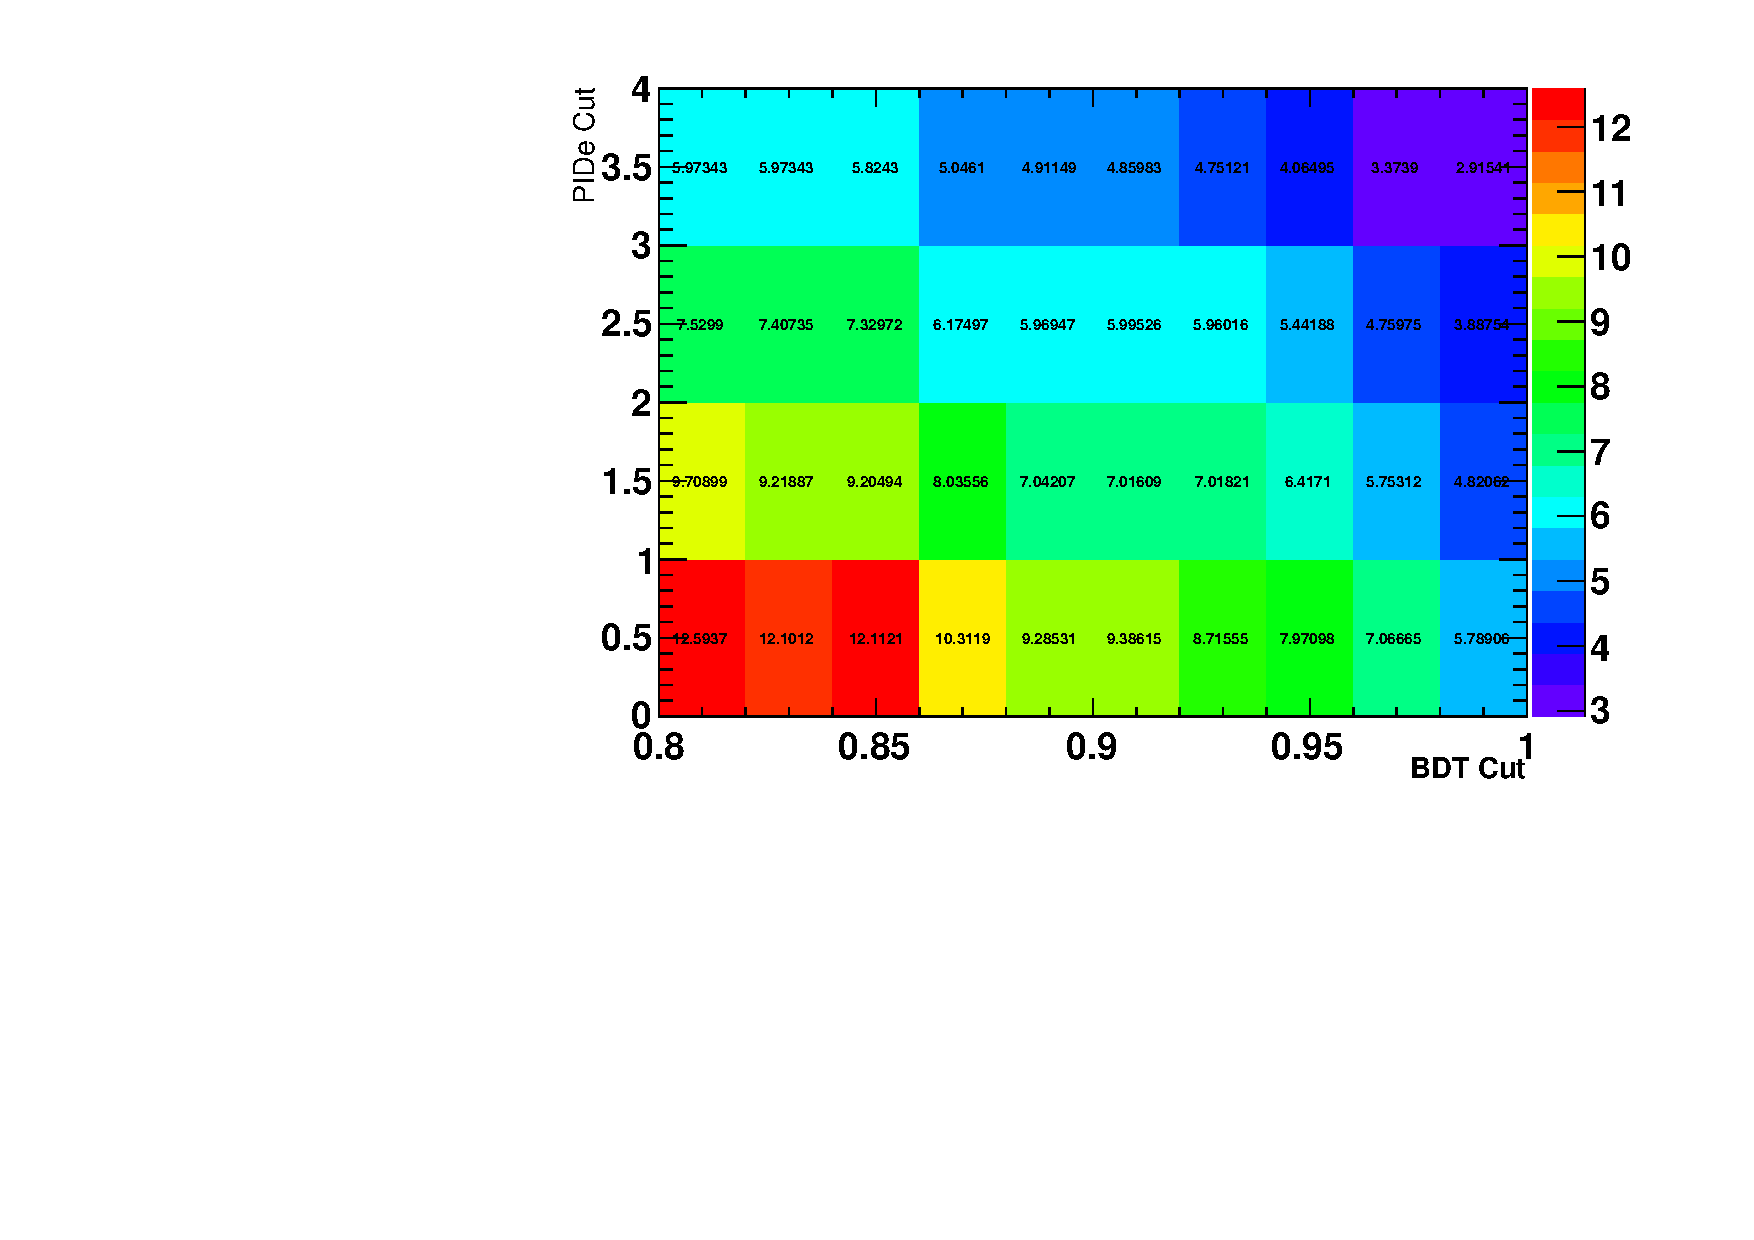
\includegraphics[width = 0.7\textwidth]{BDT_L0Had_B.pdf}}
\end{center}
\label{fig:SBHad}
\caption{\textit{Values for the expected signal yield (top) and number of background events in the signal window (bottom) for the L0Hadron trigger categories for a fourth of the 2011 and 2012 \lhcb data.}}
\end{figure}

\begin{figure}[!h]
\begin{center}
\subfigure{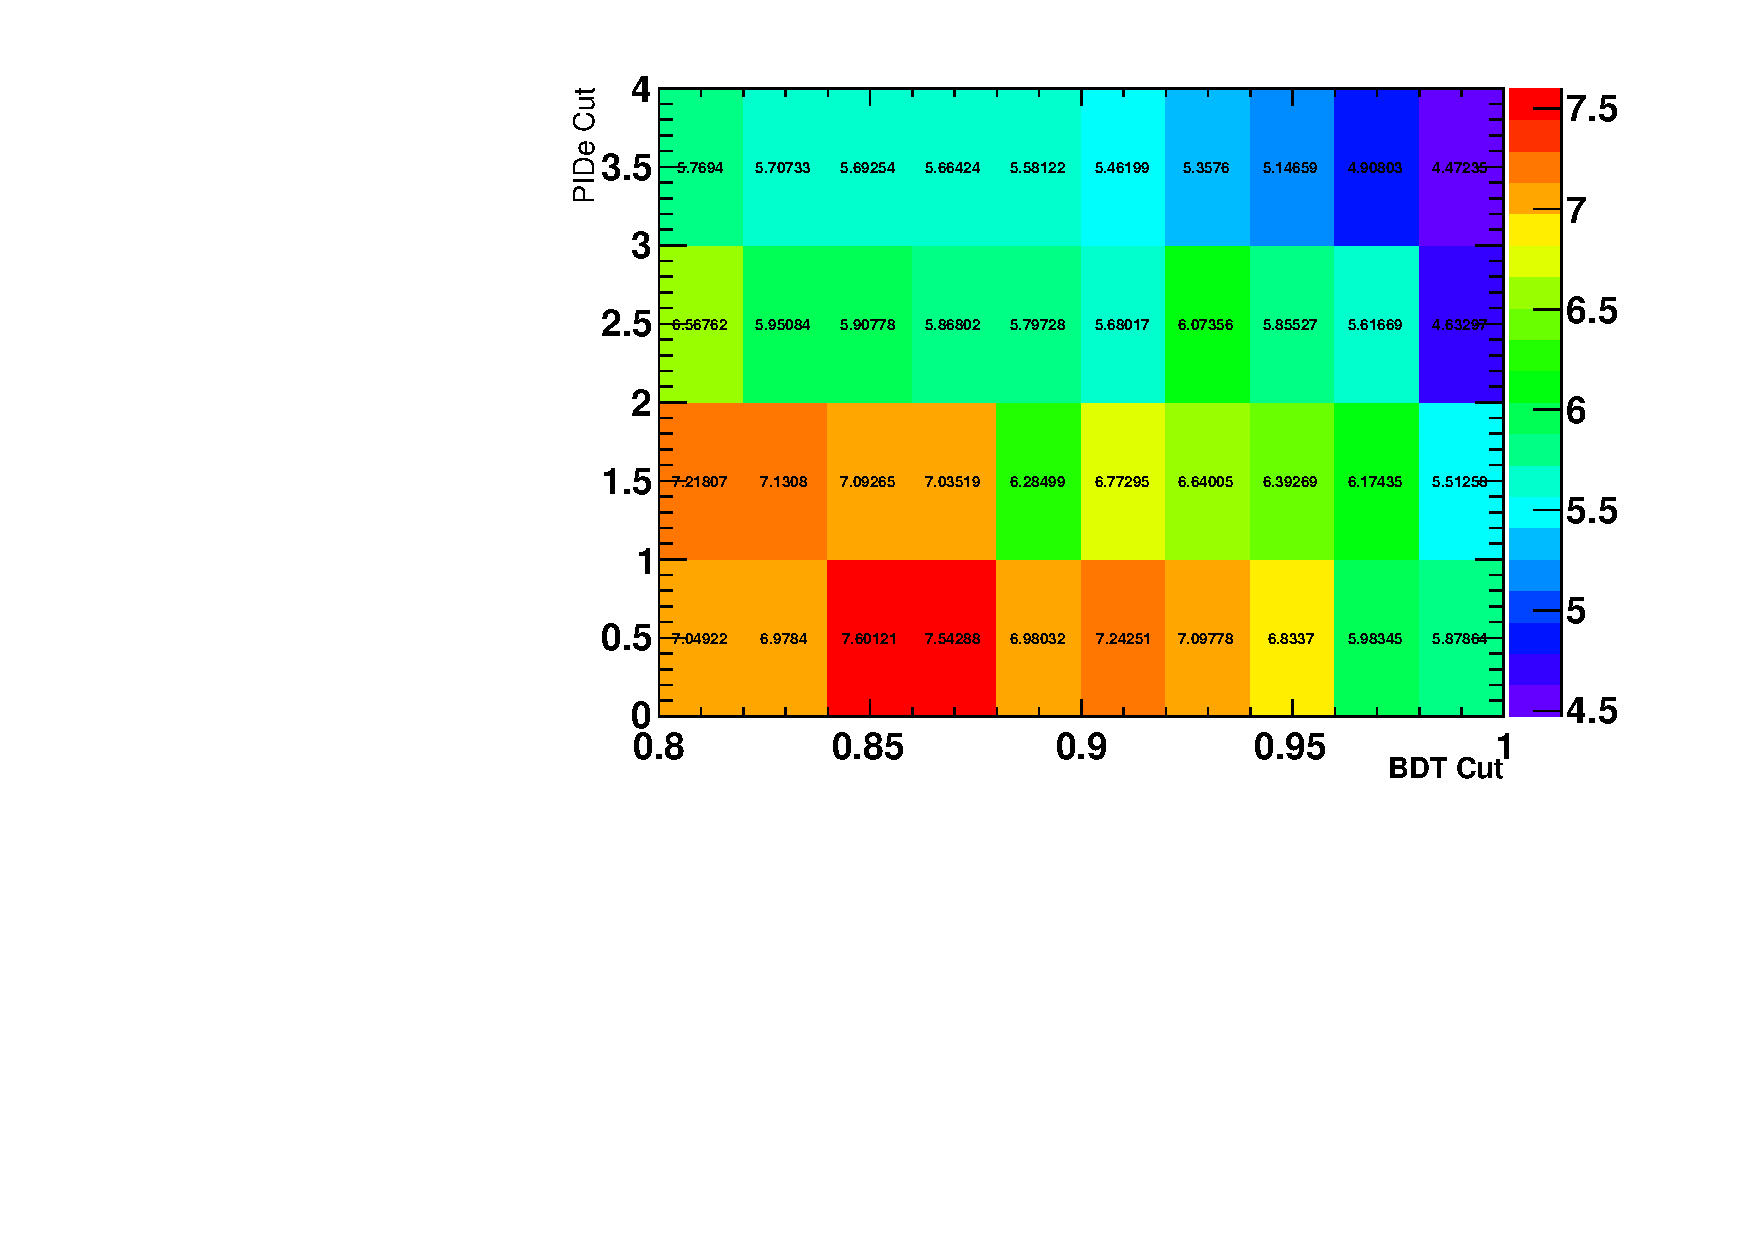
\includegraphics[width = 0.7\textwidth]{BDT_L0TIS_S.pdf}}
\subfigure{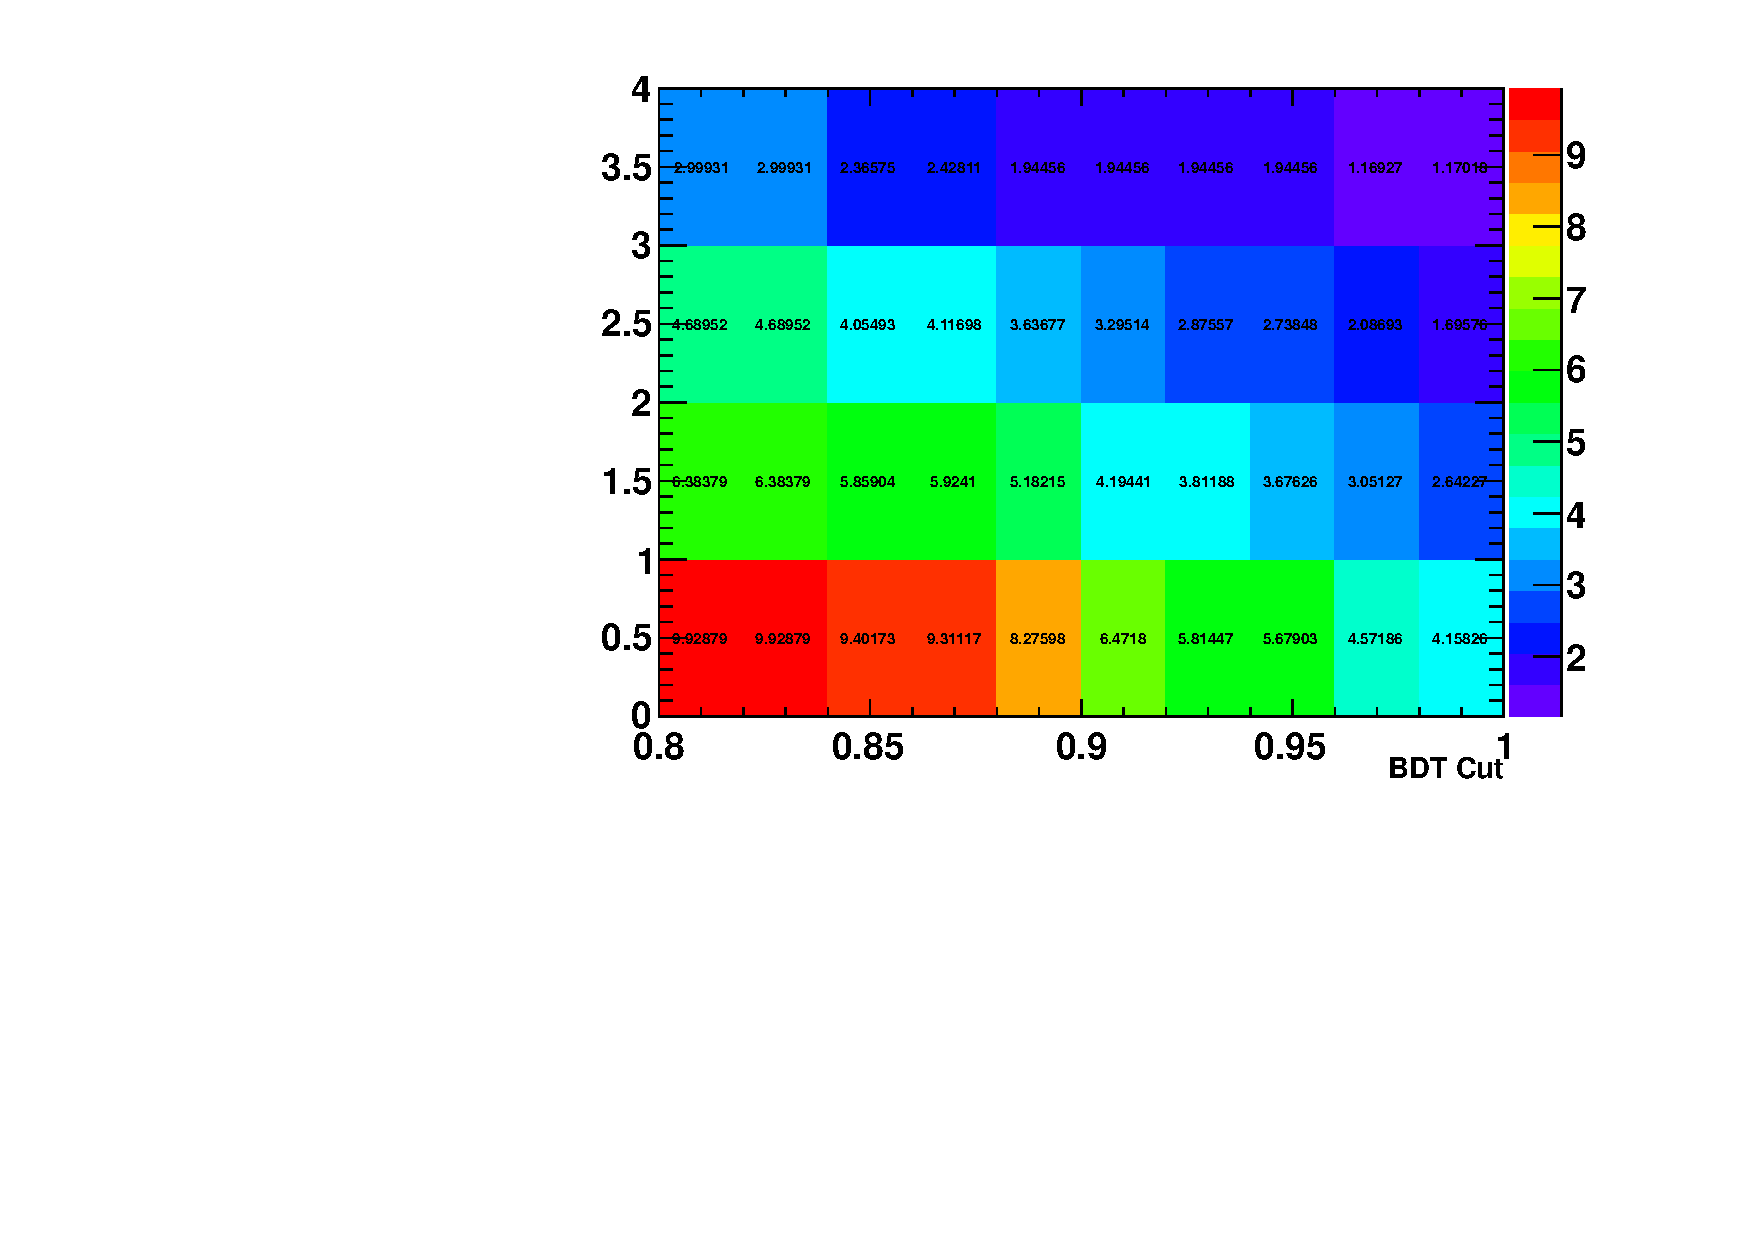
\includegraphics[width = 0.7\textwidth]{BDT_L0TIS_B.pdf}}
\end{center}
\label{fig:SBEle}
\caption{\textit{Values for the expected signal yield (top) and number of background events in the signal window (bottom) for the L0TIS trigger categories for a fourth of the 2011 and 2012 \lhcb data.}}
\end{figure}